\section{Results}

In this section, Hamiltonian embeddings for error functions of the form (\ref{eq:single-error}) and (\ref{eq:system-error}) are implemented for solving biprime factorization, polynomial SOS problems, and linear systems of equations.
For the first two problem, the focus is placed on increasing the bit precision $n$, since
it was shown in Section 4 that increasing the relative precision causes the physical energy gap $\Delta'$ to decay exponentially.
For problems with $n$ bits of precision per variable, the number of samples was assigned to $500n$ (a linear increase).
As outlined in Section \ref{sec:background}, this should maintain a (nearly) constant probability of achieving the ground state under ideal conditions.
However, since the problem conditioning is largely determined by $\Delta'$, it is somewhat concerning that the perturbations in (\ref{eq:perturbed}) could have a significant negative impact on the computation for large precision $n$.
In fact, the problem conditioning does seem to cause some significant decay in the probabilities.
However, the presented results achieve the ground state for every problem that could be embedded on the current D-Wave hardware, indicating that the primary limiting factor is the number of physical qubits $N'$ required to embed the physical Hamiltonian.

For the linear system problem, the focus is shifted to how the proposed methodology is affected by increasing the number of equations and variables, with a fixed four-bit precision.
Since there is no multiplication between variables in a linear system, the analysis results of Section 4 suggest that these types of problems should scale better on the D-Wave 2000Q hardware.
However, somewhat surprisingly, the D-Wave is unable to find exact solutions for relatively small linear systems, even when the true solution is exactly representable for the binary encoding.

\subsection{Factorization}
\label{sec:factorization}

To factor a biprime $M = x^{(1)}x^{(2)}$, where $x^{(1)}$ and $x^{(2)}$ are $n$-bit unsigned integers, the corresponding polynomial is 
$$
p\left(x^{(1)},x^{(2)}\right) = x^{(1)}x^{(2)} - M
$$
and the squared error function is given by
\begin{equation}
E\left(x^{(1)},x^{(2)}\right) = \left(x^{(1)}x^{(2)} - M\right)^2.
\label{eq:primefact}
\end{equation}
Creating $n^2$ ancillary qubits $y_{i,j} = x^{(1)}_i \wedge x^{(2)}_j$, this energy function can be embedded into a QUBO as described in Section 3.
Note that the best available techniques also require $\mathcal{O}(n^2)$ ancillary qubits for prime factorization \cite{dridi2017prime,jiang2018quantum,peng2008quantum}. 
The results for embedding this QUBO as a physical Hamiltonian (as described in Section 5) and running on the D-Wave hardware are shown in Table \ref{tab:biprime}.
Similar to the work done by Jiang et al.\ for biprime factoring, this methodology encodes $M$ directly into the Hamiltonian as a constant, rather than wasting extra qubits to store $M$ as a variable.
In fact, Jiang et al.\ used a nearly identical methodology for arbitrary integer factorization, but favored a multiplication table for factoring biprimes.


\begin{table}
    \centering
    \begin{tabular}{c|c c c|c c|c|c}
         Bits & $x^{(1)}$ & $x^{(2)}$ & $x^{(1)}x^{(2)}$ & Logical & Physical & Sq. Error & Occurrence \\ \hline
         2 & 2 & 3 & 6 & 8 & 16 & 0 & 180 \\
         3 & 5 & 7 & 35 & 15 & 69 & 0 & 311 \\
         4 & 11 & 13 & 143 & 24 & 148 & 0 & 35 \\
         5 & 29 & 31 & 899 & 35 & 349 & 0 & 82 \\
         6 & 59 & 61 & 3599 & 48 & 658 & 0 & 7 \\
         7 & 113 & 127 & 14351 & 63 & 1293 & 0 & 3 \\
         8 & 241 & 251 & 60491 & 80 & -- & -- & -- \\
    \end{tabular}
    \caption{Using the squared-error energy function methodology, biprimes with various bits of precision are factored. The columns depict the number of bits, the numbers multiplied and their product, the number of logical and physical qubits required, the minimum squared error (minimum energy) achieved by the quantum annealer, and the number of samples that produced the optimal solution. The number of samples taken grows as $500n$, where $n$ is the number of bits. Correct solutions are found for all embedded problems, however at 8-bits no physical embedding could be discovered for the logical Hamiltonian on the available the hardware. The multiplication circuit constructed with this methodology has a dense $n^2$ subgraph as well as a dense $n$ subgraph, making the number of physical qubits required to embed the Hamiltonian grow faster than the number of logical qubits on the Chimera graph structure of the available quantum annealing hardware.}
    \label{tab:biprime}
\end{table}

The most recent work in biprime factorization solves a slightly larger problem \cite{dridi2017prime,jiang2018quantum} by assuming properties of the factors.
In contrast, this methodology can factor arbitrary integers (which may not be biprimes) while still achieving the same number of bits of precision as those best known results.
As presented, arbitrary integer factorization takes the same form as biprime factorization, but has more candidate solutions (and an innately higher likelihood of success).
For that reason, only biprimes are considered here.
The correct factorization is obtained up to $M=14351$ (whose prime factors are both $7$-bit unsigned integers) by minimizing (\ref{eq:primefact}), which is also the largest problem that can be successfully embedded on current quantum annealing hardware.
At $n=8$ bits of precision, the Hamiltonian failed to embed onto the D-Wave 2000Q system, due to size limitations.

\subsection{Nonlinear Least Squares}


\begin{figure}
\centering
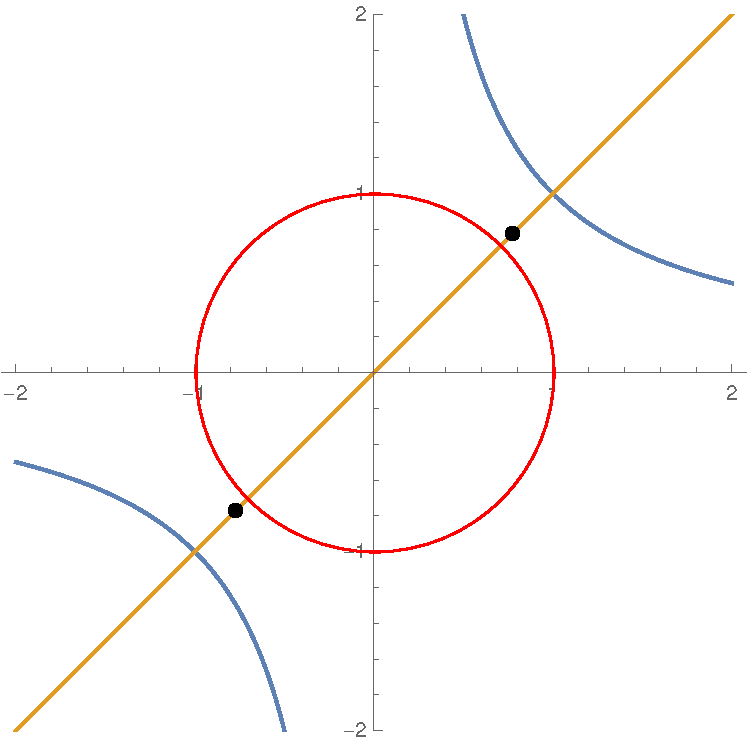
\includegraphics[width=0.9\textwidth]{fig3.pdf}
\caption{Least squares graph: this figure shows a plot of the least squares problem defined by the polynomial system of equations $xy=1$, $x^2 + y^2 =1$, and $x-y=0$.
The solutions of $(0.7746,0.7746)$ and $(-0.7746,-0.7746)$ are shown.
}
\label{fig:ls-graph}
\end{figure}

Let $\mathbf{v} = [x,y]^T \in \mathbb{R}^2$, and consider the following system of polynomial equations.
\begin{equation}
\begin{array}{rcl}
    xy &=& 1\\
    x^2+y^2 &=& 1\\
    x - y &=& 0
    \end{array}
    \label{eq:ls-system}
\end{equation}
This results in the squared energy function
$E(\mathbf{v}) = (xy-1)^2 + (x^2+y^2 - 1)^2 + (x-y)^2$.
A graph of the system (\ref{eq:ls-system}) is shown in Figure \ref{fig:ls-graph}.
To find the solution in the first quadrant, $x$ and $y$ are encoded as unsigned $n$-bit numbers each with an exponent of $e = -n$ using the encoding (\ref{eq:binary-encoding}).
The true solution is $x=y\approx 0.77$, with a minimum squared residual of $r^2 = 0.2$.
For $n=2$, the physical embedding is shown in Table \ref{tab:poly_ls_embedding}.
As seen in Table \ref{tab:poly_ls}, for $n>2$, the physical qubit requirement appears to grow super-linearly but sub-exponentially with the logical qubit requirement.

\begin{table}
    \centering
    \begin{tabular}{c|c c c|c}
      Logical Bit & Embedding &$\quad$& Logical Bit & Embedding \\ \cline{1-2}\cline{4-5}
      1 & 1376, 1383, 1248 && 6  & 1390, 1382, 1384 \\
      2 & 1380, 1379, 1251 && 7  & 1389, 1381        \\
      3 & 1261, 1258, 1253 && 8  & 1391, 1257, 1385 \\
      4 & 1249, 1377       && 9  & 1252, 1250       \\
      5 & 1388, 1386       && 10 & 1255, 1263
    \end{tabular}
    \caption{The exact embedding used in the polynomial least squares problem for $2$ bits of precision is displayed with the logical bit index in the \textit{Logical Bit} column and the physically embedded bit indices on hardware (all of which are chained to be equal) in the \textit{Embedding} column. Notice that the Chimera graph structure requires 25 physical qubits to represent the 10 logical qubits. The physical embedding was heuristically chosen using { \tt minorminer.find_embedding}, which constructed chains of 2 and 3 qubits to match the logical Hamiltonian to the connectivity of the Chimera graph. Notice also that the physical qubit indices are an automatically selected subset of the 2000 qubits available on the D-Wave 2000Q machine. The logical QUBO uses bits 1--4 to store the variables $x$ and $y$ and bits 5--10 are ancillary bits introduced through quadratization.}
    \label{tab:poly_ls_embedding}
\end{table}


%% Using embedding with 25 qubits:
%%  0 [1376, 1383, 1248]
%%  1 [1380, 1379, 1251]
%%  2 [1261, 1258, 1253]
%%  3 [1249, 1377]
%%  4 [1388, 1386]
%%  5 [1390, 1382, 1384]
%%  6 [1389, 1381]
%%  7 [1391, 1257, 1385]
%%  8 [1252, 1250]
%%  9 [1255, 1263]


The results collected on the D-Wave machine are shown in Table \ref{tab:poly_ls}.
For all tests through up to $6$ bits of precision, the closest representable solution is found.
For $n=7$ bits of precision, again, the Hamiltonian failed to embed due to size constraints.

\begin{table}
    \centering
    \begin{tabular}{c|c c|c c|c|c}
         Bits & $x$ & $y$ & Logical & Physical & Sq. Error & Occurrence \\ \hline
         2 & $3/4$ & $3/4$ & 10 & 26 & 0.2070 & 455 \\
         3 & $3/4$ & $3/4$ & 21 & 104 & 0.2070 & 50 \\
         4 & $3/4$ & $13/16$ & 36 & 286 & 0.2061 & 82 \\
         5 & $25/32$ & $25/32$ & 55 & 596 & 0.2005 & 21 \\
         6 & $25/32$ & $49/64$ & 78 & 1216 & 0.2004 & 2 \\
         7 & $99/128$ & $99/128$ & 105 & -- & -- & -- \\
    \end{tabular}
    \caption{Using the squared-error energy function methodology, a polynomial least squares problem is solved. The columns depict the number of bits of precision in the variables, the best representable solution to the least squares problem, the number of logical and physical qubits required, the minimum squared error (minimum energy) achieved by the quantum annealer rounded to 4 decimal digits, and the number of samples that produced the optimal solution. $500n$ samples were drawn from the quantum annealer for all tests, where $n$ is the number of bits of precision in the solution. In this test, the numbers are represented in fixed point notation where all bits are after the decimal. This means that the binary digits encode negative powers of two. The obtained solutions are the best possible solutions that can be achieved for their respective precision, however at 7-bits no physical embedding could be discovered for the logical Hamiltonian on the available the hardware.}
    \label{tab:poly_ls}
\end{table}


\subsection{Linear System of Equations}

Thus far, the presented results have featured an integer-valued and nonlinear problem, and focused on increasing the bit precision $n$.
In general, integer valued and nonlinear problems are interesting because they do not classically admit analytic solutions, as commented on by Chang et al. \cite{chang2019quantum}.
By contrast, as discussed by Borle et al. \cite{borle2019analyzing}, the time complexity involved in embedding linear and least squares systems of equations into a Hamiltonian rivals the time complexity of solving the system using classical techniques.
However, linear and least squares systems of equations remain interesting problems because of their wide usage in data science and applied mathematics.
Furthermore, the proposed method could still be useful in the context of large sparse systems.

In order to study how the proposed method scales with increasing numbers of variables and equations, consider a $K \times K$ linear system of equations for $K = 2,\ldots,8$.
To demonstrate signed linear algebra, one set of experiments is carried out using the two's complement binary encoding in (\ref{eq:binary-encoding}) with no bits of precision before the decimal and three bits of precision after the decimal.
To demonstrate unsigned linear algebra, another set of experiments is carried out using the unsigned binary encoding from (\ref{eq:binary-encoding}) with one bit of precision before the decimal and three bits of precision after the decimal.
The results are shown in Table \ref{tab:linear_ls}.
Note that under the proposed methodology, it is not apparently ``easier'' to solve a trivial system.
Therefore, for convenience of analysis and reproducability, the embedded system in the signed case is of the form $\mathbf{B}_0 \mathbf{v}=\mathbf{0}$, where the coefficients in the matrix $\mathbf{B}_0$ are randomly generated numbers in the range $(-1,1)$ rounded to the nearest multiple of $0.25$.
In the unsigned case, a similar system $\mathbf{B}_1 \mathbf{v} = \mathbf{c}_1$ is constructed, such that the solution is instead $\mathbf{v}=\mathbf{1}$.
All the presented problems use four bit variables, which is standard for the D-Wave 2000Q system \cite{borle2019analyzing}, and are run for $500 K$ samples.

\begin{table}
    \centering
    \begin{tabular}{c|c c|c c|c c}
         $K$ & Logical & Physical & \multicolumn{2}{c|}{\shortstack{\textit{Unsigned}\\ S.E. $\ \ $ Occ.}} & \multicolumn{2}{c}{\shortstack{\textit{Signed}\\ S.E. $\ \ $ Occ.}} \\ \hline
         2 & 8 & 22 & 0.000 & 24 & 0.000 & 2 \\
         3 & 12 & 38 & 0.000 & 23 & 0.000 & 27 \\
         4 & 16 & 80 & 0.005 & 3 & 0.013 & 1 \\
         5 & 20 & 130 & 0.026 & 1 & 0.048 & 1 \\
         6 & 24 & 202 & 0.037 & 1 & 0.048 & 1 \\
         7 & 28 & 267 & 2.604 & 1 & 1.882 & 1 \\
         8 & 32 & 312 & 0.917 & 1 & 0.767 & 1
    \end{tabular}
    \caption{Using the squared-error energy function methodology, a linear system is solved. The columns depict the number of variables \textit{and} equations in a test ($K \times K$ matrix), the number of logical and physical qubits required, the minimum squared error (minimum energy) achieved by the quantum annealer rounded to 2 decimal digits, and the number of samples that produced the best achieved solution. $500 K$ samples were drawn from the quantum annealer for all tests. In this test, the numbers are represented in $4$ bit fixed point notation with $3$ bits after the decimal. The embeddings used by the signed and unsigned systems are identical, only QUBO coefficients vary. Best achievable solution has $0$ error for all $K$.}
    \label{tab:linear_ls}
\end{table}


Note that Borle et al. \cite{borle2019analyzing} were able to solve least squares systems of size $100\times 8$ to reasonable accuracy, by increasing the annealing time from 20 microseconds (the default value) up to 50 microseconds and performing 10,000 samples.
For the experiments shown here, both the signed and unsigned linear systems are solved and an exact solution is obtained up to a system of size $3\times 3$. 
For larger systems, an inexact approximate solution is still obtained.
Although Section 4 indicates that the proposed methodology should scale better with the number of variables $d$ than with the precision $n$, these results suggest the opposite, since the only limiting factor in Sections 6.1 and 6.2 was the size of the D-Wave 2000Q machine.
It is worth noting that the physical qubit requirements in Table 3 do not challenge the size limitations.

The primary objective of these experiments is to demonstrate generality and provide an accessible method of encoding polynomial SOS problems on modern QA systems.
Although it was not demonstrated, it is reasonable to assume that improved results can be obtained by increasing the annealing time and sample count.
